%%%%%%%%%%%%%%%%%%%%%%%%%%%%%%%%%%%%%%%%%%%%%%%%%%%%%%%%%%
%  _____           _____ 
% |_   _|   /\    / ____|
%   | |    /  \  | (___  
%   | |   / /\ \  \___ \ 
%  _| |_ / ____ \ ____) |
% |_____/_/    \_\_____/ 
%                        
%%%%%%%%%%%%%%%%%%%%%%%%%%%%%%%%%%%%%%%%%%%%%%%%%%%%%%%%%%%%
% This the main document of the diploma thesis template
% Created by Ralf Wunderlich
% 
% Improvements made 
% Andreas Neyer
% Niklas Zimmermann
% Bastian Mohr
% Josua Arndt
% Ralf Wunderlich
%
% - Do not change anything in this document without the permission of your supervisor
% - Compile the document for further information
% 
% For questions and comments contact Josua Arndt
%
%%%%%%%%%%%%%%%%%%%%%%%%%%%%%%%%%%%%%%%%%%%%%%%%%%%%%%%%%%%%

\documentclass[
%draft,
paper=a4, %Seitengroesse A4
pagesize=auto,
12pt, %Schriftgroesse
twoside=true, %Doppelseitig
openright, %ein neues Kapitel beginnt immer auf einer rechten Seite
toc=bibliography, %Literaturverzeichnis wird in das Inhaltsverzeichnis aufgenommen
headsepline, %Linie unter der Kopfzeile
headinclude=true, % Kopfzeile nicht zum Textk�rper z�hlen sondern zu Randbereich
footinclude=false, % Kopfzeile nicht zum Textk�rper z�hlen sondern zu Randbereich
DIV=12, %Groesse des bedruckten Bereichs auf einer Seite. Zur Satzspiegelberechnung siehe Komascript Hilfe. Bei nichtgefallen der automatischen Satzspiegelberechnung kann auf das geometry Paket zurueckgegriffen werden. 
BCOR4mm, %Einstellung fuer den zusaetzlichen inneren Rand zur Bindekorrektur
cleardoublepage = empty, % f�gt am ende eines Kapitels eine Leerseite ein und erzwingt das fluschen von floating objekten, da scrbook ein Dokument mit doppelseitigem Layout erstellt. Style Plain nur die Seitenzahl an einer Leeren seite am ende des Kapitels. Empty ohne seitenzahl.
%parskip, % Um Absaetze mit Leerzeile zu trennen
numbers=noendperiod % Kein Punkt hinter Kapitelnummern
]
{scrbook} %KoMa-Script Ersatz der Standard-Klasse 'book'
\usepackage[]{geometry}

\setcounter{secnumdepth}{3} % Number subsubsection

\usepackage[latin1]{inputenc} % Haupts�chlich f�r Umlaute


%% Conditionals
\usepackage{ifthen} 
% True fuer den Entwurfsmodus
%\newboolean{DraftMode} % no Effect Josua
% True fuer die Druckversion
\newboolean{PrintVersion}
% True fuer die vertrauliche Version
\newboolean{ConfidentialVersion} 
\newcommand{\confidential}[2]{\ifthenelse{\boolean{ConfidentialVersion}}{#1}{#2}}
% True fuer englische Version
\newboolean{IsEnglish} 
% True for NoLogo on the firstpage
\newboolean{NoLogo}

%% Do not change the Conditionals here, 
% change them in the Settings.tex file
%\setboolean{DraftMode}{false}  % no Effect Josua
%\setboolean{PrintVersion}{false} 
%\setboolean{ConfidentialVersion}{false}
%\setboolean{IsEnglish}{false}
%\setboolean{NoLogo}{false}


\usepackage[pdftex]{graphicx, color}

%------------------------------
% Literaturverzeichnis
%-------------------------------
%  If you prefer numbers instead of recommended alphabetic use style=numeric-comp
\usepackage[style=alphabetic,natbib=true,firstinits=false, bibencoding=latin1, backend=bibtex8, url=false, backref=false]{biblatex}


%% Change the settings of the file here

%%
%\setboolean{DraftMode}{false} % no Effect Josua
% To set Packeges to draft mode go to Vorloge_DA.tex 
% and set document options to draft. Makes Compiling much faster. 

% faster PDF Generation but PDF needs much more MB 
% \pdfcompresslevel=0

% change Links and IAS Logo to Black and white Printable output.
\setboolean{PrintVersion}{true} 
% adds CONFIDANTIAL Print to Bottom line
\setboolean{ConfidentialVersion}{false}
% Changes TOC, ABR, LOF and most parts of the document to english
\setboolean{IsEnglish}{false}

% Changes First Page to use No Logo
\setboolean{NoLogo}{true}

% Please look at http://www.rwth-aachen.de/go/id/hjxv
% or search for "Hinweise zu schriftlichen Arbeiten an der RWTH" 
% to get the "Erkl�rung zur Verwendung des logos" and reache it in to "ZPA"


\newcommand{\IASAuthor}{Richter-Brockmann, Jan}
\newcommand{\IASTitleGerman}{Dokumentation des Kernel Modules f�r den LPRF Transceiver Chip}
\newcommand{\IASTitleEnglish}{Implementation and Evaluation of capacitor-based Living Object Detection in Wireless Charging of electric vehicles}
\newcommand{\IASSubject}{Bachelorarbeit}% Bachelorarbeit, Studienarbeit usw.
\newcommand{\IASMatNr}{320561}
\newcommand{\IASSupervisor}{Schrey, Moritz M.Sc.}
\newcommand{\IASNumber}{B106}
\newcommand{\IASSubmissionDate}{\today}



\graphicspath{{bilder/}} %relativer Pfad, in dem die Bilder liegen


\bibliography{mybib}



%%% Dont edit packages and other stuff from here!

\usepackage{scrhack} %kompatibilitaet von koma script mit anderen paketen herstellen

\ifthenelse{\boolean{IsEnglish}}
{
  \usepackage[english]{babel}
  \selectlanguage{english}
}
{
  \usepackage[ngerman]{babel}
  \selectlanguage{ngerman}
}
  
%--------------------------
% Schriftarten etc.
%--------------------------
\usepackage[T1]{fontenc} %Schriftkodierung auf Type1 stellen
\usepackage{textcomp} %besondere Symbole im Textmodus verfuegbar. Siehe Comprehensive Symbol List.


\usepackage{lmodern} 
\usepackage{csquotes} %anfuehrungszeichen rekonfigurierbar 
\usepackage[babel=true]{microtype} %optischer randausgleich, besserer zeilenumbruch etc.
%-------------------------------
% Seitenformatierung
%-------------------------------
\usepackage{scrpage2} %Komascript Ersatz fuer das Fancyheadings Paket
\setheadsepline{0.5pt} %Dicke der Linie unter der Kopfzeile einstellen

\usepackage{setspace} %wird zum Zeilenabstand veraendern (z.B. in der Erklaerung) gebraucht

% print out the penalty values to log
\typeout{Current Penalties:^^J
\string\clubpenalty=\the\clubpenalty^^J
\string\widowpenalty=\the\widowpenalty^^J
\string\displaywidowpenalty=\the\displaywidowpenalty}%

% Not good 
% Hurenkinder und Schusterjungen komplett verbieten.
% to forbid single.
% Disable single lines at the start of a paragraph (Schusterjungen)
% \clubpenalty = 10000
% Disable single lines at the end of a paragraph (Hurenkinder)
% \widowpenalty = 10000 
%
% Better use 
% looseness=-1 % to shorten the Paragraph one line or
% looseness=1 % to prolong the Paragraph one line or
% at the place of occurence. no space between paragraph and comand.

%-------------------------------------------
% Bilder, Formeln, Tabellen und Programmcode
%-----------------------------------------
%Bilder
\usepackage{epstopdf}  % allows to include eps graphix with includegraphics Josua
\usepackage{subfigure} %Bilder mit jeweils eigener Beschriftung nebeneinander setzen
\usepackage{pdflscape} %Seiten koennen im Landscape-Modus gesetzt werden und werden auch im Acrobat Reader um 90� gedreht dargestellt.
%\usepackage{float} % Ermoeglicht das "gewaltsame" Unterdruecken des Floatens von Figureumgebungen
\usepackage{pgfplots}
\usepackage{graphicx}
\usepackage{tikz}
\usetikzlibrary{matrix}

%\usepackage{varwidth}
%\usepackage{onimage}

\usetikzlibrary{external}
\tikzexternalize[prefix=tikzplot/]
%\tikzset{/tikz/external/optimize=false}

%Formeln
\usepackage[tbtags]{amsmath} %Tollerer Formelsatz. Fuer Befehle siehe amsldoc.pdf
\usepackage{amsfonts}
\usepackage{trfsigns} %fuer laplace transformations symbole
\usepackage{gensymb}

%Tabellen
\usepackage{array} %fuer maechtigere Tabellen
\usepackage{booktabs}   %% unterschiedliche horizontale Strichstaerken in Tabellen
\usepackage{multirow}
\usepackage{tabularx}   %% for Tubular which span the whole textwith
\usepackage{longtable} %% Multipage tables
%\setlength{\aboverulesep}{2pt}
%\setlength{\belowrulesep}{2pt}

% Graphiken, Plots, etc
\usepackage{pgfplots}

%%-----------------------------------------
%%  Pakete und Einstellungen f�r pdflatex
%%-----------------------------------------
% Changed color of links for the online version
\definecolor{blueLink}{RGB}{6,69,173}
\definecolor{lightBlueLink}{RGB}{51,102,187}
\definecolor{darkBlueLink}{RGB}{10,10,128}
\definecolor{lightGray}{RGB}{95,95,95}

\usepackage[pdfpagelayout=TwoPageRight,bookmarksopen=true,bookmarksopenlevel=1, plainpages=false, pdfpagelabels=true ]{hyperref}

\ifthenelse{\boolean{PrintVersion}}
{
\hypersetup{bookmarksnumbered=true , linktoc=all, colorlinks=false, linkbordercolor={0.02353 0.27059 0.67843}, citebordercolor={0.37255 0.37255 0.37255}, urlbordercolor={0.03922 0.03922 0.50196}, breaklinks=true} 
}
{  
  \hypersetup{bookmarksnumbered=true , linktoc=all, colorlinks=true, linkcolor=blueLink, citecolor=lightGray, urlcolor=darkBlueLink, breaklinks=true} 
}


\hypersetup{pdfauthor={\IASAuthor}, pdftitle={\IASTitleGerman}, pdfsubject={\IASSubject}}
\usepackage{pdfpages} %Zum Einbinden von ganzen pdf-Seiten (z.B. im Anhang)
\usepackage{url} %fuer URLs in der Bibliographie





%----------------------------------
%Listings
%----------------------------------
\usepackage{listings} %Fuer Programm-Quellcode im Text
%\input{listings/lstskill} % SKILL Language
%\input{listings/lstvams} % Verilog-A/AMS Language
% define colors for source code list
\ifthenelse{\boolean{PrintVersion}} %
{% Print Version - Use no colors
  \definecolor{colKeys}{gray}{0}
  \definecolor{colIdentifier}{gray}{0}
  \definecolor{colSystem}{gray}{0}
  \definecolor{colDirectives}{gray}{0}
  \definecolor{colComments}{gray}{0}
  \definecolor{colString}{gray}{0}
  \definecolor{colNumbers}{gray}{0}
  \hypersetup{colorlinks=false,final=true}  
}%
{%  Online Version - Use colors and links
  \definecolor{colKeys}{RGB}{0,46,184}
  \definecolor{colIdentifier}{RGB}{0,0,0}
  \definecolor{colSystem}{RGB}{0,46,184}
  \definecolor{colDirectives}{RGB}{0,33,133}
  \definecolor{colComments}{RGB}{0,153,0}
  \definecolor{colString}{RGB}{148,0,209}
  \definecolor{colNumbers}{RGB}{0,0,0} 
  \hypersetup{colorlinks=true,final=true}  
}
%\lstset{
%  captionpos=b,
%  abovecaptionskip=\medskipamount,
%  numbers=left,
%  numberstyle=\tiny\ttfamily\color{colNumbers},
%  language=VerilogAMS,
%  firstnumber=1,
%  frame=single,
%  frameround=fttt,
%  tabsize=4,
%  basicstyle=\small\ttfamily,
%  numberbychapter=true,
%  %escapechar=\#, % Escape char allows access to Latex. # will lead to some issues in Verilog sources
%  escapechar={}, % No escape char
%  showstringspaces=false,
%  breakatwhitespace=true,
%  breaklines=true,
%  prebreak=\raisebox{0ex}[0ex][0ex]{\ensuremath{\hookleftarrow}},
%  postbreak=\raisebox{0ex}[0ex][0ex]{\ensuremath{\hookrightarrow\space}}, %,
%  keywordstyle=[0]\bfseries\color{colKeys},         % Keyword style - VerilogXL
%  keywordstyle=[1]\bfseries\color{colKeys},         %                 Verilog-AMS/A
%  keywordstyle=[3]\bfseries\color{colSystem},       %                 System Taskts
%  keywordstyle=[4]\bfseries\color{colDirectives},   %                 Compiler Directives
%  commentstyle=\itshape\color{colComments},      % Comment style
%  stringstyle=\color{colString},         % String literal style
%  identifierstyle=\color{colIdentifier}  % Identifier Style
%}



%%-----------------------------------------
%%Einheiten
%%-----------------------------------------
\usepackage[load-configurations=binary,load-configurations=abbreviations]{siunitx} % Einbinden von SI-Einheiten  und erlaubt das direkte Setzen von SI-Einheiten wie mV
\ifthenelse{\boolean{IsEnglish}}
{\sisetup{output-decimal-marker = {.},per-mode = symbol, detect-all}}
{\sisetup{  output-decimal-marker = {,},  per-mode = symbol,  detect-all}}






%----------------------------
% Abkuerzungsverzeichnis
%----------------------------------
\ifthenelse{\boolean{IsEnglish}}
{
  \usepackage[noprefix, english]{nomencl}
  \renewcommand{\nomname}{List of Abbreviations}
}
{
  \usepackage[noprefix, german]{nomencl}
  \renewcommand{\nomname}{Abk�rzungsverzeichnis}
}
\setlength{\nomlabelwidth}{0.2\hsize} %Abstand zwischen Abk. und Erklaerung
\setlength{\nomitemsep}{-\parsep} %Abstand zwischen Eintraegen
\let\abk\nomenclature
% Punkte zw. Abk�rzung und Erkl�rung
\setlength{\nomlabelwidth}{.15\hsize}
\renewcommand{\nomlabel}[1]{#1 \dotfill}
% Zeilenabst�nde verkleinern
%\setlength{\nomitemsep}{-\parsep}
\makenomenclature

%% Index erstellen mit 
%% makeindex Vorlage_DA.nlo  -s nomencl.ist -o Vorlage_DA.nls


%------------------------------
% Sonstiges
%-------------------------------
\hyphenation{Gate-ox-id Code nie-der-oh-mig} %Vorgaben fuer Silbentrennungen



\interfootnotelinepenalty 10000
%%------------------------------------------
%%  Dokumentenanfang
%%------------------------------------------
\begin{document}
  \frontmatter % Vorspann der Arbeit, roemische Seitennummerierung
  
  \begin{titlepage}

\pagestyle{empty}

\ifthenelse{\boolean{IsEnglish}}
{
\pdfbookmark[0]{Front Page}{Front Page} %Titelseite in die pdf-Bookmarks aufnehmen        
}
{
\pdfbookmark[0]{Titelseite}{Titelseite} %Titelseite in die pdf-Bookmarks aufnehmen    
}

% set textheight so the date also fits when Tittles get bigger
\enlargethispage{2.3in}
% set topmargin so picture fits in Page
\setlength{\voffset}{-1in}

\ifthenelse{\boolean{NoLogo}}
{
   \vspace*{32.4mm} 
}
{ 
\ifthenelse{\boolean{PrintVersion}}
{  \hspace*{4.5cm}\includegraphics[height=32mm, trim= 5 5 50 5 ]{Logos_2015/rwth_ias_bild_schwarz_grau_cmyk.eps}
}
{
  \hspace*{4.5cm}\includegraphics[height=32mm, trim= 5 5 50 5 ]{Logos_2015/rwth_ias_bild_rgb.eps}
}\bigskip 
}\setcounter{subfigure}{0}

~\\
Lehrstuhl f�r Integrierte Analogschaltungen
der RWTH Aachen. \bigskip \\ \bigskip
~\\~\\~\\~\\
{\Large \bfseries \IASTitleGerman\\} \bigskip 
~\\~\\~\\~\\
%{\Large \bfseries \IASTitleEnglish\\} \bigskip
% 
%% bring the next text down to the bottom so variation of title lenght don�t change the position of this text
%\par\vspace*{\fill}
%~\\
%{\Large \IASSubject\\}\bigskip
%
%~\\
{\Large von\\~\\}~{\Large \IASAuthor\\}~\\
{\Large und\\~\\}~{\Large Schrey, Moritz\\} 
%{\Large Matr.-Nr. \IASMatNr\\} \bigskip \bigskip

%~\\
%{\large Unter Betreuung von \IASSupervisor\\} \bigskip \bigskip 
%
%~\\
%{\Large 1. Pr�fer: Prof. Dr.-Ing. Stefan J. Heinen}
%~\\
%{\Large 2. Pr�fer: Prof. Dr. sc. techn. Renato Negra}
%\confidential{\vspace*{0.8cm}}{\vspace*{1.3cm}}
%\confidential{\vspace*{0.4cm}}{\vspace*{1.1cm}}
%\confidential{~\\
%\ifthenelse{\boolean{IsEnglish}}
%  {\textbf{CONFIDENTIAL}}
%  {\textbf{VERTRAULICH}}
%  }{}
%
%\centerline{ \Large \IASNumber}
\vspace*{\fill}
\centerline{ \Large Aachen, \IASSubmissionDate}

\newpage
% reset the voffset so the following pages have the Normal Layout
\setlength{\voffset}{0in}

\thispagestyle{empty}
\rule{0pt}{0pt}
\cleardoublepage
\end{titlepage}
               %Titelseite einf�gen
  \cleardoubleemptypage
  \pagestyle{plain}
  \tikzexternaldisable
  %\includepdf[]{Anhang/Erkl�rungBA.pdf}
  \tikzexternalenable
  %\input{Erklaerung.tex}           %Datei Erklaerung.tex einfuegen  
  %\input{danksagung.tex}      
  % Table of content
  \BeforeTOCHead[toc]{{\cleardoublepage\pdfbookmark[0]{\contentsname}{toc}}} %Inhaltsverzeichnis in pdf bookmarks
  \pagestyle{plain}    %Seitennummerierung, aber keine Kopfzeile
  \tableofcontents    %Inhaltsverzeichnis erstellen

%%--------------------------------
% Verzeichnisse
%%---------------------------------
  % Figures
  \cleardoublepage\phantomsection\addcontentsline{toc}{chapter}{\listfigurename}
  \listoffigures
  % Tables
  \cleardoublepage\phantomsection\addcontentsline{toc}{chapter}{\listtablename}
  \listoftables
  % Listings
  \cleardoublepage\phantomsection\addcontentsline{toc}{chapter}{Listings}
  \lstlistoflistings
  % Abbrevations
  \ifthenelse{\boolean{IsEnglish}}
  {
    \cleardoublepage\phantomsection\addcontentsline{toc}{chapter}{List of Abbreviations}
  }
  {
    \cleardoublepage\phantomsection\addcontentsline{toc}{chapter}{Abk�rzungsverzeichnis}
  }
  \printnomenclature

%%--------------------------------
% Hauptteil
%%---------------------------------
  \mainmatter
  \pagestyle{scrheadings}
  \ifthenelse{\boolean{IsEnglish}}
  {
    \confidential{\cfoot{\textbf{CONFIDENTIAL}}}{}
  }
  {
    \confidential{\cfoot{\textbf{VERTRAULICH}}}{}
  }  
  
  % Add the content of the file here

% lprf driver 

\chapter{LPRF Driver}

\section{Strukturierung der Dateien}

Alle Dateien, die zu dem LPRF Treiber geh�ren, befinden sich im Repository \textit{https://github.com/ias-aachen/lprf-driver}. In Tabelle \ref{tab:dateien} sind diese Dateien mit ihren zugeh�rigen Funktionen aufgelistet. 

\begin{table}[hbtp]
  \centering      
  \begin{tabular}{ll}
  \toprule
             Datei								& Funktion          \\
  \midrule
             load\_driver.sh 					& Skript zum Einbinden des Treibers, nimmt alle \\ 
             										& n�tigen Einstellungen vor \\           
  \midrule	
             lprf.h				      		& Header-Datei f�r das Modul, viele struct Definitionen                 	\\  
  \midrule
             lprf\_tx.c			   			& Implementierung des Treibers, eigentlicher Code     								\\
  \midrule
 			    lprf\_tx.ko           			& Datei wird zum Einbinden des Treibers ben�tigt									\\
  \midrule
 			    Makefile              			& Enth�lt die Regeln f�rs Compilen														\\	
  \midrule
 			    output\_dmesg\_lprf.txt		& Ausgabe des dmesg nach einem Sendevorgang 											\\				
  \midrule
 			    userspace.c						& Erm�glicht das Auslesen eines Registers des \\
 			    										& Chips bei laufendem Betrieb	\\	
  \midrule 
  				 lprf\_registers.h					& Enth�lt die Register Definitionen \\   
  \bottomrule
  \end{tabular}
        
   \caption{Zugeh�rige Dateien zum LPRF Treiber\label{tab:dateien}}   
\end{table}

Das Einbinden des LPRF Treibers geschieht �ber den Befehl \textit{\$sudo insmod lprf\_tx.ko}. Daf�r muss das Module kompiliert sein und eine \textit{*.ko} Datei existieren. Um das Ausbinden, Kompilieren und wieder Einbinden zu erleichtern, ist es m�glich, das Skript \textit{load\_driver.sh} aufzurufen. Dort werden alle n�tigen Schritte f�r eine Benutzung des Treibers durchgef�hrt. Dies beinhaltet auch das Erstellen einer Ger�tedatei unter \textit{/dev}, welches mit dem Befehlt \textit{\$sudo mknod /dev/lprf c 243 0} geschieht. Zum Schluss wird das WPAN Device gestartet. Die dazu notwendigen Dateien befinden sich im Verzeichnis \textit{/lprf-driver/ieee802154}.


\section{Beschreibung des Codes}

\subsection{Wichtige structs}

In dem Treiber wird viel mit Structs gearbeitet, welche oft auch untereinander verkn�pft sind. Dieses Kapitel soll �ber die wichtigsten verwendeten Structs einen �berblick geben. 

\subsubsection{lprf\_local}

Der Struct \textit{lprf\_local} (Listing \ref{lis:local}) dient dem Speichern aller Daten �ber das Device. Dazu z�hlen die Einstellungen f�r die SPI Kommunikation, das regmap Subsystem, boolesche Variablen und structs von Typ \textit{lprf\_state\_change} (dazu mehr in \ref{sec:StructStateChange}). Dieser Struct dient daher auch der Kommunikation zwischen den Funktionen. 

\begin{lstlisting}[language={C}, caption=Struct lprf\_local, label=lis:local]
struct lprf_local {
	struct spi_device *spi;

	struct ieee802154_hw *hw;	
	struct lprf_chip_data *data;
	struct regmap *regmap;
	int slp_tr;

	struct completion state_complete;
	struct lprf_state_change state;

	bool tx_aret;
	unsigned long cal_timeout;
	s8 max_frame_retries;
	bool is_tx;
	bool is_tx_from_off;

	u8 tx_retry;
	struct sk_buff *tx_skb;
	struct lprf_state_change tx;

	struct lprf_state_change rx;
	struct lprf_state_change debug;
};

\end{lstlisting}


\subsubsection{lprf\_state\_change}\label{sec:StructStateChange}

Der Struct \textit{lprf\_state\_change} wird f�r die Kommunikation zwischen den Funktionen, welche vom IEEE802.15.4 Layer aufgerufen werden, benutzt. Damit in solchen Funktionen auch der Struct \textit{lprf\_local} zur Verf�gung steht, wird dieser ebenfalls in \textit{lprf\_state\_change} verkn�pft. Des Weiteren enth�lt der Struct Informationen �ber ben�tigte Timer, den Buffer (dort werden die Bytes der SPI Kommunikation abgelegt) und boolesche Werte �ber einen Statuswechsel. 

\begin{lstlisting}[language={C}, caption=Struct lprf\_state\_change, label=lis:stateChange]
struct lprf_state_change {
	struct lprf_local *lp;

	struct hrtimer timer;
	struct spi_message msg;
	struct spi_transfer trx;
	u8 buf[LPRF_MAX_BUF];

	void (*complete)(void *context);
	u8 from_state;
	u8 to_state;
};

\end{lstlisting}


\subsubsection{lprf\_chip\_data}

In Listing \ref{lis:chipData} ist die Implementierung des Structs \textit{lprf\_chip\_data} dargestellt. Dieser enth�lt haupts�chlich die Zeiten, welche die verschiedenen Komponenten auf dem Chip zum Einschwingen ben�tigen. Alle Zeiten werden in $\mu s$ angegeben. 

\begin{lstlisting}[language={C}, caption=Struct lprf\_chip\_data, label=lis:chipData]
struct lprf_chip_data {
	u16 t_from_sleep_to_tx;
	u16 t_from_tx_idle_to_tx;
	u16 t_from_rx_power_to_tx;
	u16 t_from_rx_pll_to_tx;
	
	u16 t_from_sleep_to_rx;
	u16 t_from_tx_to_rx;
	u16 t_from_rxhold_to_rx;

	u16 t_from_sleep_to_txidle;
	u16 t_from_tx_to_txidle;
	u16 t_from_rx_to_txidle; 
	u16 t_from_rx_pll_to_txidle;

	u16 t_from_sleep_to_rxhold;
	u16 t_from_tx_to_rxhold;
	u16 t_from_rx_to_rxhold;

	
	int rssi_base_val;

	int (*set_channel)(struct lprf_local *, u8, u8);
	int (*get_desense_steps)(struct lprf_local *, s32);
};
\end{lstlisting}



\subsubsection{ieee802154\_ops}

In dem Struct \textit{ieee802154\_ops} werden Funktionspointer zu all den Funktionen abgelegt, welche vom IEEE802.15.4 Layer ben�tigt und aufgerufen werden. Die wichtigsten f�r den LPRF Treiber sind die Funktionen \textit{int (*start)(struct ieee802154\_hw *hw)} und \textit{int (*xmit\_async)(struct ieee802154\_hw *hw, struct sk\_buff *skb)}. Wann diese Funktionen aufgerufen werden und welchen Nutzen sie haben wird, weiter unten in Kapitel \ref{sec:lprf_start} und \ref{sec:lprf_xmit} erl�utert. 

%\begin{lstlisting}[language={C}, caption=Struct ieee802154\_ops, label=lis:ieeeOps]
%struct ieee802154_ops {
%	struct module   *owner;
%	int             (*start)(struct ieee802154_hw *hw);
%	void            (*stop)(struct ieee802154_hw *hw);
%	int             (*xmit_sync)(struct ieee802154_hw *hw, struct sk_buff *skb);
%	int             (*xmit_async)(struct ieee802154_hw *hw, struct sk_buff *skb);
%	int             (*ed)(struct ieee802154_hw *hw, u8 *level);
%	int             (*set_channel)(struct ieee802154_hw *hw, u8 page, u8 channel);
%	int             (*set_hw_addr_filt)(struct ieee802154_hw *hw, struct ieee802154_hw_addr_filt *filt, unsigned long changed);
%	int             (*set_txpower)(struct ieee802154_hw *hw, s32 mbm);
%	int             (*set_lbt)(struct ieee802154_hw *hw, bool on);
%	int             (*set_cca_mode)(struct ieee802154_hw *hw, const struct wpan_phy_cca *cca);
%	int             (*set_cca_ed_level)(struct ieee802154_hw *hw, s32 mbm);
%	int             (*set_csma_params)(struct ieee802154_hw *hw, u8 min_be, u8 max_be, u8 retries);
%	int             (*set_frame_retries)(struct ieee802154_hw *hw, s8 retries);
%	int             (*set_promiscuous_mode)(struct ieee802154_hw *hw, const bool on);
%};
%\end{lstlisting}


\subsubsection{regmap\_config}

F�r die Konfiguration des regmap Subsystems wird der Struct \textit{regmap\_config} ben�tigt. Hier werden alle Hardware- und Treiber-spezifischen Einstellungen vorgenommen. Weitere Details befinden sich im Anhang \ref{sec:regmap}.



\subsection{lprf\_probe()}

Die Funktion \textit{lprf\_probe()} wird automatisch beim Einbinden des Moduls vom Kernel aufgerufen. Hier wird zu Beginn ein Struct vom Typ \textit{ieee802154\_hw} erstellt, welcher alle notwendigen Informationen �ber die Hardware beinhaltet. Diese Daten werden dann im Struct \textit{lp} vom Typ \textit{lprf\_local} abgelegt. Dieser struct spielt in dem gesamten Treiber eine wichtige Rolle, da dieser in jeder Funktion zur Verf�gung steht (auch wenn \textit{lp} nicht mehr lokal initialisiert werden sollte). Nun folgt eine Initialisierung f�r das regmap Subsystem. Dieses wird f�r das Lesen und Schreiben von einzelnen Registern ohne Callback-Funktion genutzt. Au�erdem steht ein Debugging Modus zur Verf�gung. 

Die Funktion \textit{lprf\_setup\_spi\_messages()} dient zum Einstellen der SPI Kommunikationen. Eine besondere Rolle spielt hier der struct \textit{lprf\_state\_change}. Davon sind aktuell vier St�ck in \textit{lp} definiert. Je nach dem welche Aufgabe der Treiber gerade erf�llt, werden hier andere Implementierungen verwendet. Alle Funktionen, die vom IEEE802.15.4 Layer aufgerufen werden, bekommen einen solchen Struct als Parameter �bergeben und haben somit wieder Zugriff auf \textit{lp} (siehe Listing \ref{lis:stateChange}). 

Als n�chster Schritt wird die Funktion \textit{lprf\_detect\_device()} aufgerufen. Diese liest die Chip ID Register (RG\_CHIP\_ID\_H und RG\_CHIP\_ID\_L) aus und pr�ft diese auf korrekten Inhalt (0x1A und 0x51). Falls einer der Werte nicht korrekt ausgelesen wird, wird der Initialisierungsprozess des LPRF Treibers abgebrochen. Am Ende von \textit{lprf\_detect\_device()} werden noch Hardware-spezifische Einstellungen vorgenommen. Genaueres l�sst sich aus den Kommentaren im Code entnehmen. 

Nun werden zwei Initialisierungsfunktionen f�r die Verwendung der Completion-Struktur und der SPI Kommunikation aufgerufen. Dabei handelt es sich um \textit{init\_completion()} und \textit{spi\_set\_drvdata()}. 

Der nun folgende Aufruf von der Funktion \textit{lprf\_hw\_init()} dient f�r das Setzten aller notwendigen Register. Mit der dort verwendeten Funktion \textit{lprf\_write\_subreg()} werden nur einzelne Bits ge�ndert. Die Funktion \textit{\_\_lprf\_write()} hingegen �ndert den gesamten Wert eines Registers und wurde verwendet, wenn mehrere Bits in einem Register ge�ndert werden mussten. Diese wurden dann zu einem Wort zusammengefasst und in einem Schreibvorgang aktualisiert. 

Zum Abschluss in \textit{lprf\_probe()} wird der Char-Driver initialisiert (dazu weiter unten mehr) und die Hardware im IEEE802.15.4 Layer registriert. Daf�r finden die Funktionen \textit{scull\_init\_module()} und \textit{ieee802154\_register\_hw()} Anwendung. 






\subsection{lprf\_start()}\label{sec:lprf_start}

Die Funktion \textit{lprf\_start()} wird durch den IEEE802.15.4 Layer aufgerufen, wenn ein WPAN Netzwerk �ber den Treiber initialisiert wird (\textit{/ieee802154/setup\_wpan.sh}). Zur Zeit erf�llt der Aufruf dieser Funktion keinen weiteren Nutzen. Ein m�glicher Verwendungszweck k�nnte allerdings die Implementierung einer Polling-Struktur f�r den RX-Pfad sein. 





\subsection{lprf\_xmit()}\label{sec:lprf_xmit}

Wenn mit dem User Space Programm \textit{/ieee802154/client\_udp\_802154.c} auf den Treiber zugegriffen wird, wird die Funktion \textit{lprf\_xmit()} aufgerufen und ein Sendevorgang gestartet. Um einen aktiven Sendevorgang zu kennzeichnen, wird der boolesche Wert \textit{lp->is\_tx} auf logisch 1 gesetzt. Au�erdem werden die zu �bertragenden Daten vom IEEE802.15.4 Layer �bergeben und in \textit{lp->tx\_skb} abgelegt. Nun wird die Funktion \\ 
	\hspace*{15mm}\textit{lprf\_xmit\_start()} \\
genutzt, um lediglich die Funktion \\
	\hspace*{15mm}\textit{lprf\_write\_frame()} \\
aufzurufen. Hier werden die Bits der einzelnen zu sendenden Bytes mit der Funktion \textit{lprf\_reverse\_bit\_order()} in der Reihenfolge getauscht. Dann werden diese Daten mittels \textit{spi\_async()} an die Hardware �bertragen. Als Callback-Funktion wird \\
	\hspace*{15mm}\textit{lprf\_write\_frame\_complete()} \\
aufgerufen. Hier wird zuerst der FIFO mode aktiviert (SR\_FIFO\_MODE\_EN) und im Anschluss mit \textit{lprf\_async\_read\_reg()} das Register RG\_SM\_STATE ausgelesen. Da dieses Auslesen �ber die Funktion \textit{spi\_async()} geschieht, gibt es auch hier eine Callback-Funktion, welche in diesem Fall \\
	\hspace*{15mm}\textit{lprf\_check\_state\_complete()} \\ 
ist. Hier wird mit dem ausgelesenen Wert gepr�ft, ob die State Machine busy ist. Falls das der Fall sein sollte, wird das Register SM\_STATE erneut gelesen und als Callback-Funktion wiederum \textit{lprf\_check\_state\_complete()} aufgerufen. Wenn sich die State Machine nicht in dem Status STATE\_BUSY befindet, wird mittels der Funktion \\
	\hspace*{15mm}\textit{lprf\_get\_state()} \\ 
der ausgelesene Wert aus SM\_STATE dem passenden Status aus SM\_MAIN zugewiesen und damit der aktuelle Status der State Machine ermittelt. Dieser Status wird dann in \textit{ctx->from\_state} abgelegt. Im Anschluss wird mit der Funktion \\
	\hspace*{15mm}\textit{lprf\_async\_state\_change()} \\
ein Statuswechsel gestartet. Hier werden als Parameter der Zielstatus und eine Completion-Funktion �bergeben. Der Zielstatus wird unter \textit{ctx->to\_state} abgespeichert und die Completion-Funktion unter \textit{ctx->complete}. Danach wird das Register SM\_MAIN ausgelesen, indem wieder die Funktion \textit{lprf\_async\_read\_reg()} verwendet wird. Dieses mal wird als Callback-Funktion von \textit{spi\_async()} die Funktion \\
	\hspace*{15mm}\textit{lprf\_async\_state\_change\_start()} \\
aufgerufen. Das Auslesen aus SM\_MAIN wird gemacht, damit die letzten vier Bits aus dem gelesenen Byte selektiert werden k�nnen. Diese werden bei dem Schreiben des neuen Status ben�tigt, um ein �berschreiben dieser zu verhindern. Der Schreibprozess wird auch hier mit \textit{spi\_async()} durchgef�hrt. Als Callback-Funktion ist \\
	\hspace*{15mm}\textit{lprf\_state\_delay()} \\
definiert. Hier wird �ber eine switch-case Anweisung die korrekte Wartezeit ermittelt, um sicherzustellen, dass alle Module auf dem Chip eingeschwungen sind. Falls eine dieser Wartezeiten angepasst werden muss, kann dies �ber die Konstanten in Listing \ref{lis:TimingConst} geschehen (definiert in \textit{lprf\_registers.h}). 


\begin{minipage}{\linewidth}
	\begin{lstlisting}[language={C}, caption=Definition der Wartezeiten, label=lis:TimingConst]
	// settling times PLL
	#define T_POWER_TX_TIME		0x20
	#define T_POWER_RX_TIME		0x20
	#define T_PLL_PON_TIME		0x60
	#define T_PLL_SET_TIME 		0x60
	#define T_TX_TIME			0x40
	#define T_PD_EN_TIME		0x20
	\end{lstlisting}
\end{minipage}


Wenn die richtige Wartezeit ermittelt wurde, wird ein Timer gestartet, welcher als Callback-Funktion \\
	\hspace*{15mm}\textit{lprf\_state\_timer()} \\
aufruft. Nun wird erneut das Register SM\_STATE mittels \textit{lprf\_async\_read\_reg()} ausgelesen und als Callback-Funktion \\
	\hspace*{15mm}\textit{lprf\_async\_state\_assert()} \\
�bergeben. Hier findet mit Hilfe des ausgelesenen Wertes eine Abfrage nach Abbildung \ref{fig:TXassert} statt. 

\begin{figure}[htbp!]
	\center
  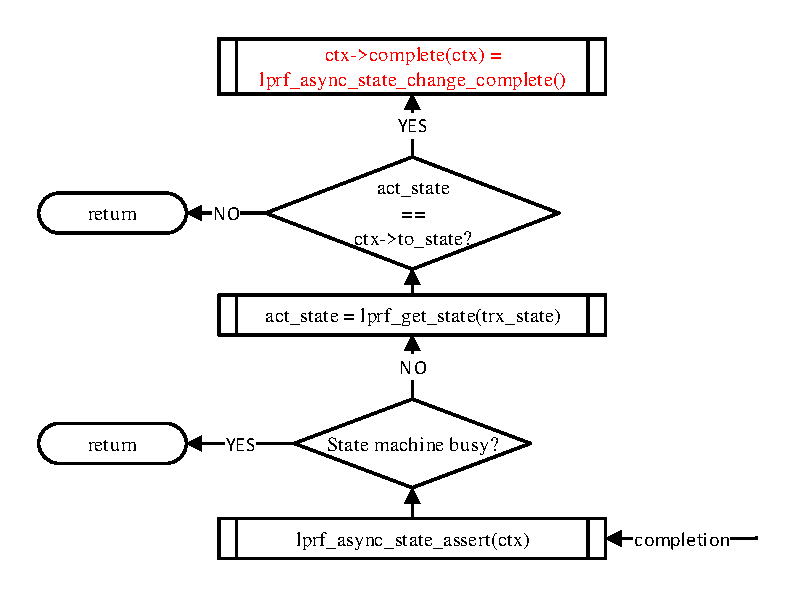
\includegraphics[width = 0.6\textwidth]{LPRF_TX_assert.pdf}
        \caption{Abfrage in \textit{lprf\_async\_state\_change()}\label{fig:TXassert}}
\end{figure} 

Mit dieser Abfrage wird �berpr�ft, ob der Statuswechsel erfolgreich war. Bei einem auftretenden Fehler wird zur Zeit nichts unternommen, sondern nur mittels \textit{return} die Funktion verlassen. Wenn allerdings alles erfolgreich durchgef�hrt wurde, wird die Funktion \\
	\hspace*{15mm}\textit{lprf\_async\_state\_change\_complete()} \\
aufgerufen (wurde in \textit{lprf\_async\_state\_change unter \textit{ctx->complete} gespeichert}). Hier wird zuerst �berpr�ft, ob \textit{lp->is\_tx} gesetzt ist. Mittels einer �berpr�fung, ob sich die State Machine noch im Sendemodus befindet, wird \textit{lprf\_async\_read\_reg()} solange aufgerufen, bis dies nicht mehr der Fall sein sollte. Dann ist das Senden beendet und das Register SM\_MAIN kann zur�ckgesetzt werden und der FIFO Mode ausgeschaltet werden. Au�erdem wird \textit{lp->is\_tx} auf logisch 0 zur�ckgesetzt. Zum Abschluss einer �bertragung �ber den IEEE802.15.4 Layer muss die Funktion \textit{ieee802154\_xmit\_complete()} ausgef�hrt werden. 





% Char Driver 

\chapter{Char Driver}

Ein Char Driver zeichnet sich durch die Kommunikation zwischen dem Kernel und dem User Space aus. Es ist also m�glich Daten vom und zum User Space zu �bertragen. 

Im LPRF Treiber wird die Implementierung eines Char Drivers genutzt, um Registerwerte im laufenden Betrieb des Chips auszulesen. Dies erm�glicht ein leichteres Debuggen des Treibers. 
\urlstyle{same}


Wie bereits oben erw�hnt, wird der Char Driver mit Hilfe der Funktion \textit{\url{scull\_init\_module()}} in \textit{lprf\_probe()} initialisiert. 


\section{scull\_read()}

Um die Verbindung zwischen User Space und Kernel Module zu schaffen, spielt die Funktion \textit{scull\_read()} eine wichtige Rolle. Damit diese Funktion allerdings Daten an den User Space zur�ckgeben kann, muss dort eine Ger�tedatei mit der zum Treiber geh�rigen Major Number erstellt werden (\textit{sudo mknod /dev/lprf -c MajorNumber MinorNumber}). Im Anschluss ist es m�glich, diese Datei auszulesen und der Char Driver liefert an diese einen Wert zur�ck. Falls das Auslesen einfach �ber \textit{\$cat} geschieht, wird in dem hier vorliegendem Fall immer das erste Register ausgegeben. Um die Registeradresse frei zu w�hlen, kann das Programm \textit{userspace.c} genutzt werden. 


Wenn die Ger�tedatei vom User Space aus ausgelesen wird, wird in dem Char Driver die Funktion \textit{scull\_read()} ausgef�hrt (Listing \ref{lis:scullRead}). Der Parameter \textit{*buf} enth�lt die Informationen �ber den Ort, von dem die Funktion aufgerufen wurde. Somit kann der Treiber die Daten an den korrekten Ort im User Space zur�ck liefern. Mit der Variable \textit{*f\_pos} wird die Adresse des auszulesenden Registers festgelegt. Dieser Pointer kann im User Space mit der c-Funktion \textit{fseek} modifiziert werden. 


\begin{lstlisting}[language={C}, caption=Implementierung scull\_read(), label=lis:scullRead]
ssize_t scull_read(struct file *filp, char __user *buf, size_t count, loff_t *f_pos)
{
	ssize_t retval = 0;
	unsigned int myval = 1;
	unsigned int dev_size = 2 + *f_pos;
	unsigned int rc;
	struct lprf_state_change *ctx = &(lp->debug);

	printk(KERN_DEBUG "lprf: scull_read - start.");
	
	// read from hardware via spi_sync()
	lprf_sync_read_reg_debugging(lp, *f_pos, ctx, 0);

	// get read value
	myval = ctx->buf[2];	
	
	count = 1;			
	
	rc = copy_to_user(buf, &myval, count);	
	if (rc) {		//1 char is transfered, count = 1	
		retval = -EFAULT;
		goto out;
	}
	
	*f_pos += count;	//+= 1
		
	if (*f_pos + count > dev_size){		
		count = dev_size - *f_pos;
		printk(KERN_DEBUG "lprf: scull_read: count=%u\n", count);
		return 0;
	}

	retval = count;

out:
	printk(KERN_DEBUG "lprf: scull_read - end. %s:%i\n", __FILE__, __LINE__);	
	return retval;
	return 0;
}
\end{lstlisting}

F�r das Auslesen des Registers wird die Funktion \textit{lprf\_sync\_read\_debugging()} verwendet. Diese spezielle Funktion ist notwendig, damit bei der SPI Kommunikation der Code des LPRF Treibers unterbrochen wird und nicht weiter ausgef�hrt wird. Ansonsten w�rde \textit{scull\_write} fortgesetzt werden, wenn noch keine ausgelesenen Daten in ctx->buf[2] vorliegen w�rde. 

Nachdem das entsprechende Register ausgelesen wurde, ist es m�glich den Wert aus {ctx->buf[2]} in \textit{myval} zu speichern. Zum Schluss kann der Wert an den User Space zur�ckgegeben werden, wozu die Funktion \textit{copy\_to\_user()} genutzt wird. 



%\input{beispiel.tex}
%%%% Add your chapters here

\printbibliography[heading=bibintoc]

\appendix


% Anhang 

\chapter{Anhang}

\section{Flow Chart - TX Pfad}
\begin{figure}[htbp!]
  \includegraphics[width = \textwidth]{LPRF_TX.pdf}
        \caption{Flow Chart �ber den TX Pfad\label{fig:FlowChartTX}}
\end{figure}



\section{Linux - Kernel Subsystem for peripheral devices}\label{sec:regmap}
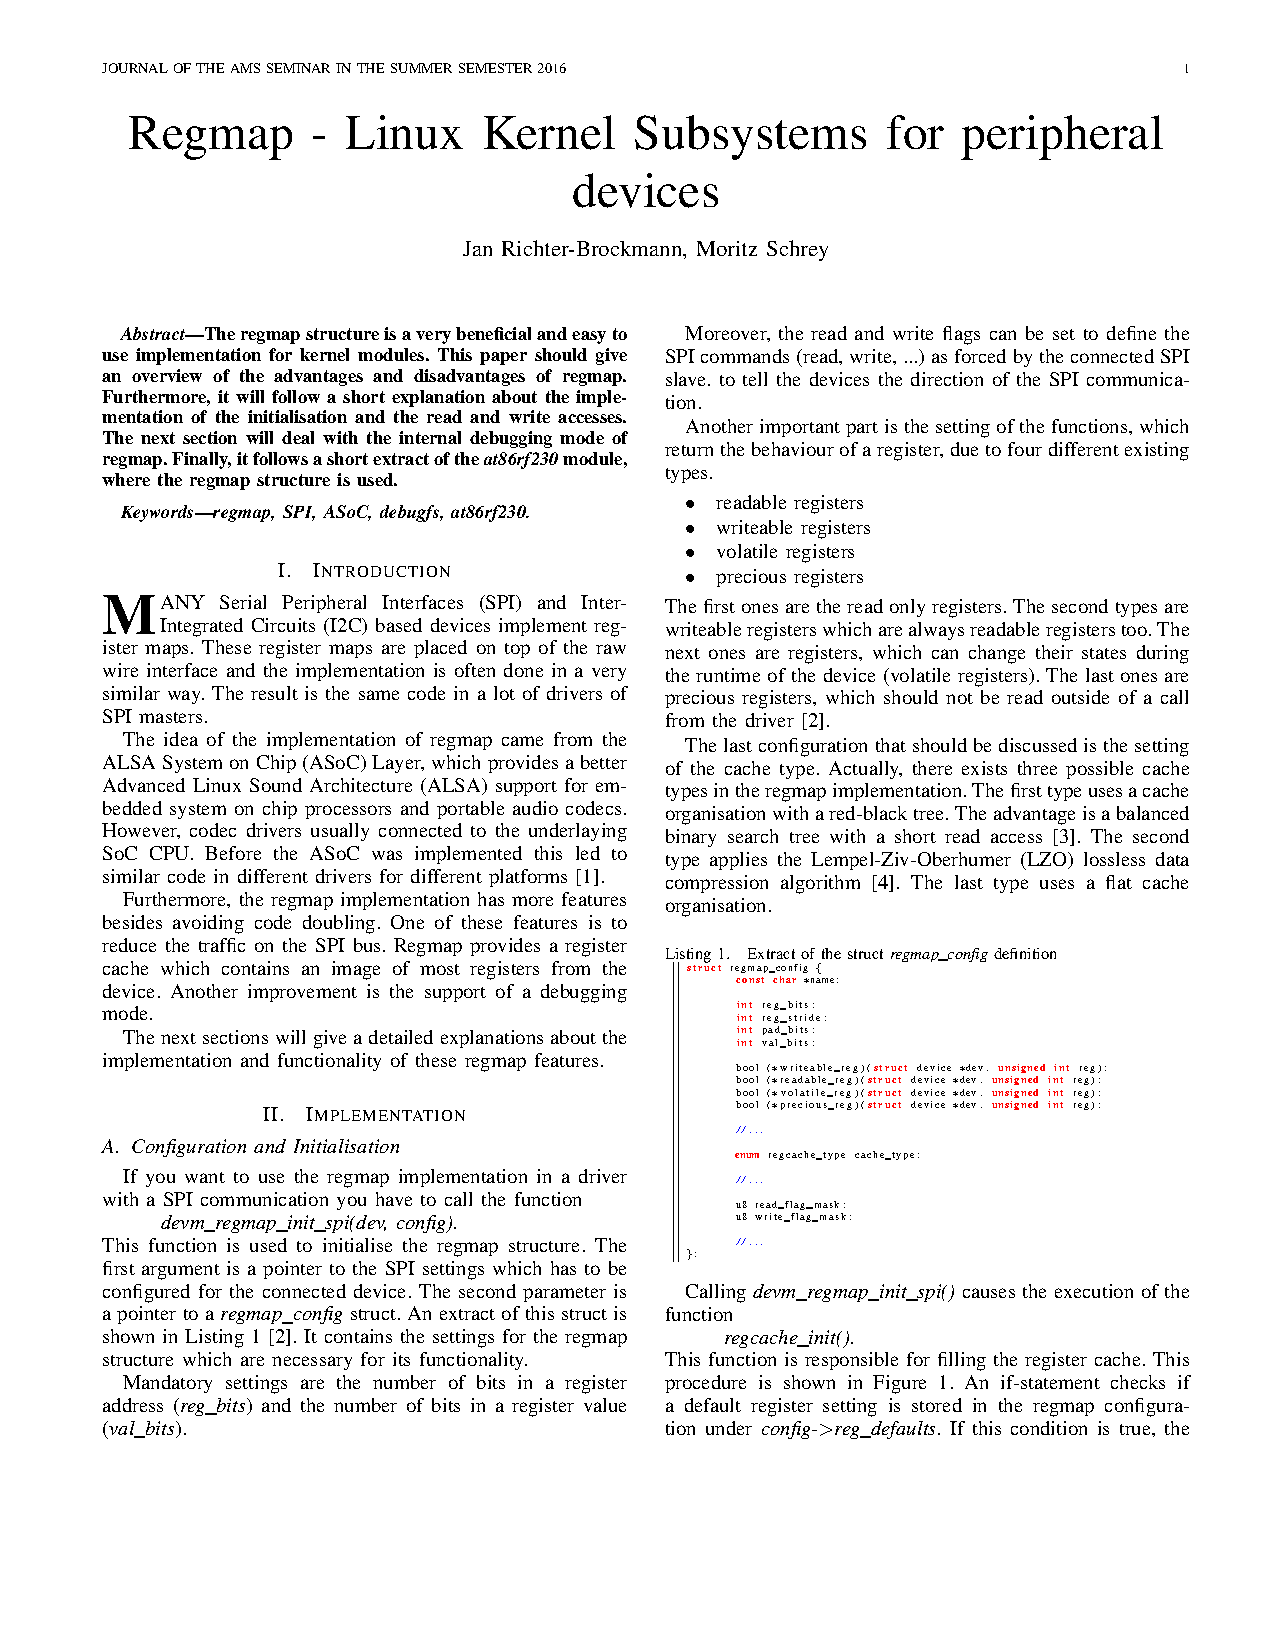
\includepdf[pages={1-5}]{Anhang/Paper_regmap.pdf}


\section{How to setup the Raspberry Pi}
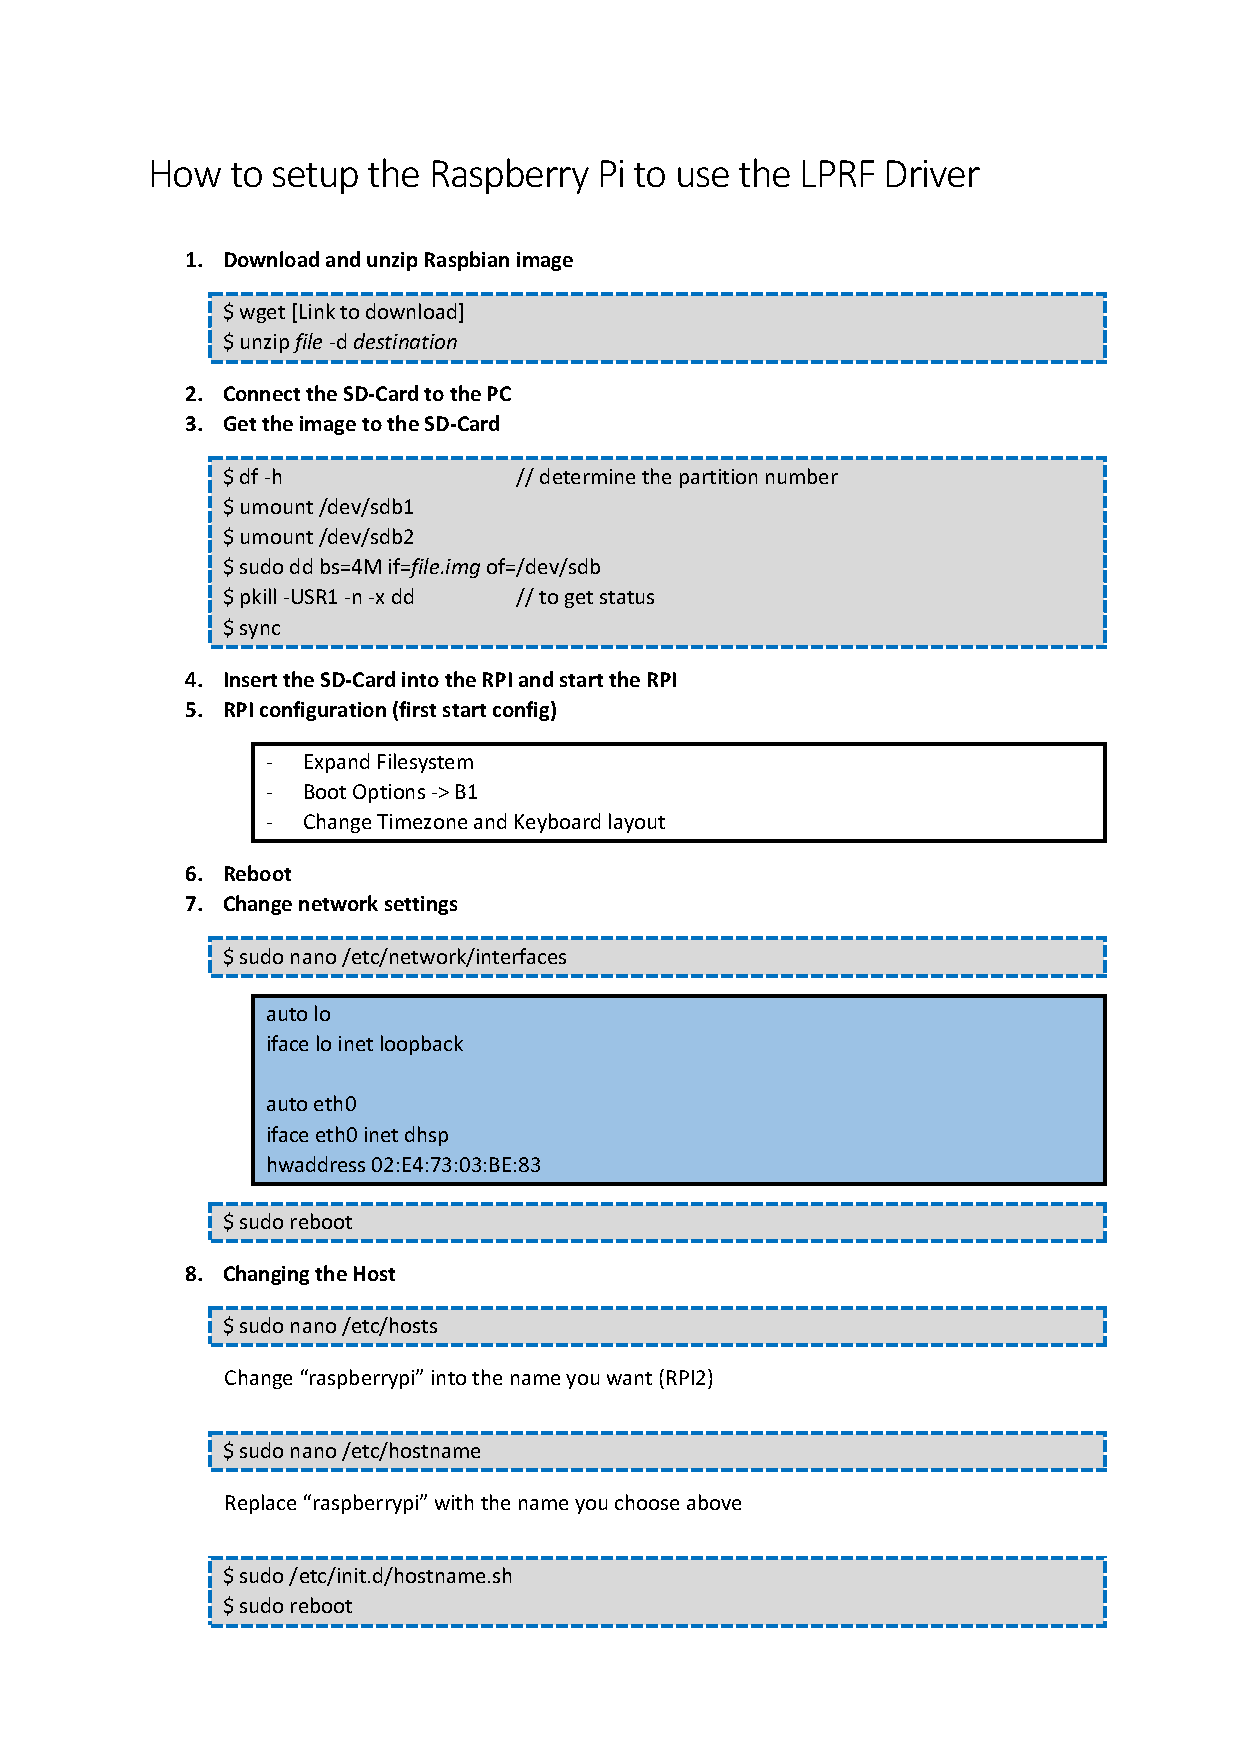
\includepdf[pages={1-6}]{Anhang/HowToSetupRPI.pdf}

%\section{Flow Chart - TX Pfad}
%\includepdf[pages={1}]{Anhang/LPRF_TX.pdf}



%
%\ifthenelse{\boolean{IsEnglish}}
%{
%  \chapter{Presentation Slides}
%}
%{
%  \chapter{Vortragsfolien}
%} 
%
%% include slides be aware of the slide numbers at include pdf page, at the beginning the chapter heading will be included so only 4 slides fit at this page. first page slide 1-4 , than include the other Pages from 5 - xx
%\tikzexternaldisable
%
%\begin{minipage}{\textwidth}
%     \includepdf[nup=2x2,pages={1-4},width=0.48\textwidth, offset=0 -3.0cm, delta=17.58pt 2cm,pagecommand={\section{Einf�hrungsvortrag}}]{../Anhang/Einfuehrungsvortrag.pdf}
%\end{minipage}
%
%\includepdf[nup=2x3,pages={5-29},width=0.48\textwidth, offset=-6.55mm 0cm, delta=17.58pt 2cm,pagecommand={\pagestyle{scrheadings}}]{../Anhang/Einfuehrungsvortrag.pdf}
%\cleardoublepage % do NOT remove
%
%
%% Final Presentation
%% No chapter Heading so no minipage
%
%%\includepdf[nup=2x3,pages={1-33},width=0.48\textwidth, offset=-6.55mm 0cm, delta=17.58pt 2cm,pagecommand=\section{Abschlussvortrag}}]{../Anhang/FinalPresentation_final.pdf}
%%\cleardoublepage % do NOT remove
%
%\begin{minipage}{\textwidth}
%     \includepdf[nup=2x2,pages={1-4},width=0.48\textwidth, offset=0 -3.0cm, delta=17.58pt 2cm,pagecommand={\section{Abschlussvortrag}}]{../Anhang/FinalPresentation_final.pdf}
%\end{minipage}
%
%\includepdf[nup=2x3,pages={5-27},width=0.48\textwidth, offset=-6.55mm 0cm, delta=17.58pt 2cm,pagecommand={\pagestyle{scrheadings}}]{../Anhang/FinalPresentation_final.pdf}
%\cleardoublepage % do NOT remove
%
%\tikzexternalenable





\end{document}
